\subsubsection[BDI]{BDI$^{\blacktriangle,\diamond/\circ}$}\label{fun:BDI}
Using cognitive modelling techniques for agent development enable autonomous behaviour and reasoning for automated problem solving.
This also allows the analysis of real world behaviour through simulations with agents.
Problems can hence be automatically solved through self-organised groups of agents and new knowledge can be drawn from such simulations.
The beliefs, desires and intentions (short: \emph{BDI}) model, is a widespread software model for developing intelligent agents situated in complex and dynamic environments.
There, the basic characteristics of an agents' mental state are expressed through beliefs, desires and intentions which are explained in more detail later in this section.
The BDI logic system is quite easy to implement in software agents and to some extent promises human-like reasoning behaviour.
Hence, it has been widely used in the field of artificial intelligence in computer science.
This section begins with the roots of the BDI model by mentioning the scientific papers that led to it.
It then continues with an explanation of practical reasoning after which the components of the BDI model are presented in greater detail.

In 1987, Bratman~\cite{MICHAEL_PlansResource_1988} discussed the relationship between beliefs, desires, intentions and actions as well their roles in agent behaviours.
This can be seen as the introduction of the BDI model which was revised in 1991 by Rao and Georgeff~\cite{rao_modeling_1991}.
They formalised the model to a first order logic and treated beliefs, desires and intentions as three modal operators while giving intentions equal importance compared to beliefs and desires.
Rao and Georgeff then continued to apply this theoretical foundation to concrete BDI agents, applying them in an airline traffic management application~\cite{Rao_BDITheory_1995}.
Nowadays, BDI agents are deployed in high technology industrial areas such as space shuttle development.
For example, PRS~\cite{Ingrand_PRS_1992} and dMARS~\cite{Mark_dMARS_2004} are both BDI-based systems for the reaction control system of the NASA Space Shuttle Discovery.

The philosophical views of the BDI model can be found in Bratman's theory of practical reasoning~\cite{Sebastian_Hierarchical_2006}.
Practical reasoning involves two important processes: deciding what goals should be achieved, and how they should be achieved.
The former process is known as \emph{deliberation}, the latter as \emph{means-ends reasoning}~\cite{Gerhard_MultiSystem_1999}.
Means-ends reasoning is a method to make plans for achieving goals based on current states.
A \emph{plan} is a strict order of actions needed to be executed to achieve a goal.
The idea of means-ends reasoning is to reduce the difference between the current state and the state where a goal is achieved.
For this purpose, the method is applied recursively.
When an agent is placed in an environment, it should autonomously decide what to do and how to do it.
In general, an agent could execute many different actions but maybe only a few of them would have a desired effect on the environment.
Various external properties can have influence on the feasibility of achieving the agent's goals.
The deliberation process filters what options are actually possible in the current state.
It then determines which of these options will become intentions.
For example, if you are thirsty and standing in a supermarket, then you might be faced with the decision to choose a drink.
There can be a lot of options like wine, beer, water, lemonade or juice.
However, picking up a bottle of wine or beer is not allowed in Germany for people under the age of 16. % Germany, sadly a proud nation of drunkards.
After collecting all the available options, you must choose and commit to some of them which become intentions next.
Subsequently, we need the mean-ends reasoning process to plan how to achieve these intentions.
If your intention is to buy a bottle of water, you may then plan to go to the shelf with water on it, reach for such a bottle, take it to the checkout counter and pay for it.
Finally, you have to execute this plan to buy the bottle of water.

The BDI model, as an applicable theory of practical reasoning, consists of three components which are beliefs, desires and intentions.
These are subsequently explained each.

Beliefs represent the informational part of the agent~\cite{Rao_BDITheory_1995} and are updated appropriately after each sensing action.
They may be implemented as a variable, a database, a set of logical expressions or some other data structure~\cite{Rao_BDITheory_1995}.
Beliefs model the agent's look at the world.
They can express information about the environment, other agents or the agent itself.
An agent may update its beliefs at any time.
Agents receive new information from the perception of the environment and the execution of intentions.
An agent can use sensors to perceive the environment and store their output as beliefs.
Beliefs are not the same concept as knowledge.
Knowledge is the realisation of a fact whereas a belief models \enquote{knowledge} which is believed by the agent.
Beliefs do not necessarily have to be true from a global perspective.
But from the agent's perspective, they are.
Hence, beliefs can be seen as local knowledge.
Likewise, beliefs can be global knowledge when they are true in a global sense.

Desires represent the motivational part of the agent~\cite{Rao_BDITheory_1995}.
In other words, desires represent objectives or situations that the agent would like to accomplish or bring about.
Desires can be but do not need to be achieved.
% Although similar, desires can be distinguished from goals.
Multiple desires can be inconsistent with each other and the agent does not need to know the means of achieving these desires.
These desires are filtered within the agent's deliberation process, therefore a subset of both consistent and achievable desires which usually called \emph{goals} are chosen by the agent~\cite{Gerhard_MultiSystem_1999}.
For example, sleeping and working may be both one's desires, but they can not both be one's goals at the same time because they conflict with each other.

Intentions are desires or actions that an agent committed itself to achieve~\cite{Alejandro_LearnBDI_2004}.
Their meaning is stronger than that of desires.
Desires are merely wishes that may be achieved or may be not, but intentions are decided to be achieved to a reasonable extent.
Michael Wooldridge~\cite{Gerhard_MultiSystem_1999} concluded four functions of intentions in practical reasoning:
\begin{itemize}
  \item Intentions driving means-ends reasoning means that intentions have decisive influences on the actions which the agent will execute.
    Agents are expected to determine ways of achieving intentions.
  \item Intentions constrain future deliberation.
    This means that options which would be in conflict with an already chosen intention will not be considered.
  \item Intentions persist means that intentions will not be given up unless there is a rational reason to do so.
    This is important because if an agent immediately dropped its intentions without devoting resources to achieving them, it will never achieve anything~\cite{Gerhard_MultiSystem_1999}.
    Hence, intentions are committed desires which can not be easily abandoned.
    A reason to drop an intention nevertheless could be e.g. when an external event made the intention impossible or a lot more difficult to achieve.
  \item Intentions influence beliefs upon which future practical reasoning is based.
    This expresses that an intention is believed to be eventually achieved under \enquote{normal circumstances}.
    Practically, after deciding on an intention, the agent will add the intention as a belief.
    This allows the agent to plan for the future on the assumption that the intention will be achieved.
\end{itemize}
Intentions play an important role in the BDI model as they lead to actions and influence future beliefs and intention selection.

Beliefs, desires and intentions are the foundation of BDI agents.
Yet, further components are needed to build the connection between these three components and thereby implement BDI agents.
Naturally, the architecture of BDI agents differs in detail depending on their tasks.
However, they all share a core architecture which is depicted in \autoref{fig:bdi_architecture}.
Its components are explained in the following paragraphs.
\begin{figure}[htbp]
  \centering
  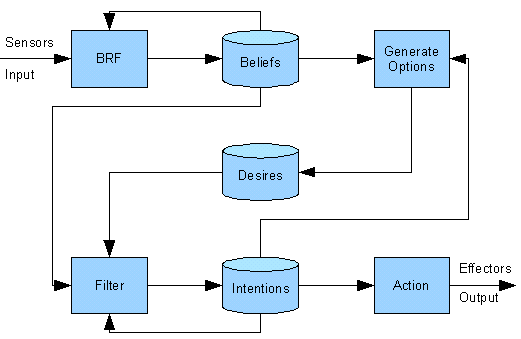
\includegraphics[width=\textwidth]{images/BDIAr}
  \caption{Brief BDI architecture~\cite{BDIA}. Squares symbolise functions whereas the elliptic shapes symbolise data sets. Arrows indicate data transmission.}
  \label{fig:bdi_architecture}
\end{figure}

The sensors of a BDI agent perceive the environment and convert the perceptions $P$ to signals as inputs for the \emph{belief revision function}.
This function collects the external perceptions as well as the beliefs which are already stored in the beliefs.
It then processes the information and updates the beliefs accordingly.
The belief revision function prefers minimal change over modifying a lot and hence tries to preserve as much information as possible~\cite{Antje_SpatialBelief_2011}.
While processing the new and old information, the belief revision function will also solves inconsistencies, e.g.\ when an agent perceives information which contradicts a belief it has.

The \emph{belief set}'s data may be modelled as sentences, rules or some other manifestations.
Formally, we denote the belief set with the letter $B$.
In the \emph{AGM approach} (named after their proponents, Alchourrón, Gärdenfors, and Makinson)~\cite{alchourron_revision_1985}, an agent's beliefs are modeled by a deductively closed set of formulas called a \emph{belief set}~\cite{James_revise_2011}.
This approach is broadly used in belief revision research.
It makes several postulates for one revision operator which mapping each belief set and one sentence of beliefs to generate new beliefs.
Meanwhile, these postulates allow the belief revision process to retain as many previous beliefs as possible to reduce the amount of change.

The \emph{option generator} commits a list of desires into the \emph{desire set} $D$.
It determines the desires depending on the agent's current beliefs and current intentions.
The desire set contains desires, which express the agent's wishes it wants to achieve.
Next, the filter determines the agent's intentions depending on the current beliefs, desires, and intentions.
Only achievable and rational desires will then become intentions.

The \emph{intention set} $I$ stores the agent's current focus, which is accompanied by a concrete plan.
Once an intention is adopted, hence stored in the intention set, the agent will pick and commit to one intention in order to achieve it.
The \emph{action selection function} determines the actions to perform depending on the current intentions.
This function draws its knowledge from a plan library which is not depicted in \autoref{fig:bdi_architecture}.
Finally, the matching plan is inspected for the next action $A$ to be executed by the agent.

\begin{table}[!hbp]
  \label{tab:BDIC}
  \begin{tabularx}{\textwidth}{|l|p{5cm}| >{$}X<{$} |}
  \hline
  \textbf{Component} & \textbf{Meaning} & \textbf{Formalisation} \\
    \hline
    Belief set & Information about the environment which the agent is located in & B \\
    \hline
    Belief revision function & Determines a new set of beliefs depending on perceptual inputs and the agent's current beliefs & B \times P \to B\\
    \hline
    Options generation function & Determines desires depending on the agent's current beliefs and current intentions & B \times I \to D \\
    \hline
    Desire set & Are states which an agent wishes to bring about & D \\
    \hline
    Filter function & Determines the agent's intentions depending on current beliefs, desires, and intentions & B \times D \times I \to I \\
    \hline
    Intention set & The agent's current focus & I \\
    \hline
    Action selection function & Determines an action to perform depending on current intentions & I \to A  \\
    \hline
  \end{tabularx}
  \caption{Meaning and formalisation of the components of the BDI agent architecture}
\end{table}
\autoref{tab:BDIC} summarises the BDI agent architecture as described by Michael Wooldridge~\cite{Gerhard_MultiSystem_1999}.
The process of $B \times P \to B$, $B \times I \to D$ and $B \times I \times D \to I$ belongs to deliberation.
They are deliberated gradually, so the range of intentions is narrowed down.
This happens especially due to the filter function which operates on all of the datasets.
$I \to A$ can be treated as the process of means-ends reasoning as the difference between the committed intention and the current situation decreases.
$B,D$ and $I$ are connected through functions instead of being connected directly.
This is because they are treated simply as functionless databases on which algorithms may work.

Although the BDI model has been introduced about 30 years ago, it is still a field of on-going development.
The BDI model restricts itself to the three main components: beliefs, desires and intentions.
In some situations, not all the three attributes are needed.
However, for some distributed multi-agents, only three attributes may not be sufficient.
One problem here is for example that the BDI model does not capture communication between agents or interaction between them.

Beliefs, desires and intentions were introduced in this section.
The BDI agent belongs to the kind of intelligent agents which are autonomous, computational entities.
They follow the practical reasoning theory.
Different BDI implementations show different architectures, but the core of these agents is most of the time built by beliefs, desires and intentions.

With an increasing number of BDI applications, more challenges come up too.
One of such challenges is the correctness of agents' behaviour.
It is described in the following \autoref{fun:formal_methods}.
